\documentclass[a4paper,12pt,oneside,final]{extbook}

\usepackage[utf8]{inputenc}
\usepackage[T1]{fontenc}

\usepackage{graphicx}
\usepackage{times}
\usepackage[english,swedish]{babel}

\usepackage{geometry}

\geometry{
 margin=20mm
} 

\usepackage{fancyhdr}

\usepackage{titling}
\title{Bruse - en webbdatabas för filhantering\\Projektrapport, TNM094}
\author{Grupp J\\Erik Olsson\\Ronja Grosz\\Klas Eskilson\\Daniel Rönnkvist\\Therése Komstadius}

\frenchspacing
\setlength{\parindent}{0pt}
\parskip 5pt

\setcounter{secnumdepth}{3}

\usepackage{color}
\definecolor{rltred}{rgb}{.5,0,0}
\definecolor{rltgreen}{rgb}{0,.5,0}
\definecolor{rltblue}{rgb}{0,0,1}

\usepackage[pdftex,
 colorlinks=true,
 urlcolor=rltblue,       % \href{...}{...} external (URL)
 filecolor=rltgreen,     % \href{...} local file
 linkcolor=rltred,       % \ref{...} and \pageref{...}
 citecolor=rltgreen,     % \cite{...}
 pdftitle={},
 pdfauthor={},
 pdfsubject={Projektrapport, TNM094},
 pdfkeywords={},
 pdfpagemode=,
 pdfstartview=FitH,
 bookmarks=true,
 bookmarksopen=false,
 bookmarksnumbered=true
        ]{hyperref}


\begin{document}

\pagestyle{empty}
\thispagestyle{empty}

\frontmatter

\maketitle

\pagestyle{fancy}

\chapter{Sammanfattning}
Den här rapporten beskriver hur en webbdatabas för filhantering utvecklades i kursen Medietekninskt Kandidatprojekt, TNM094, vid Linköpings universitet. Syftet med projektet var att gruppen skulle följa ett agilt arbetssätt för att uppnå kundens krav. Kundens främsta krav var att databasen skulle användas för att lagra och strukturera personlig information som dokument, bilder och musik. Dessa filer skulle sedan taggas med ett eller flera nyckelord för att kunna söka reda på informationen snabbare. Serversystemet utvecklades i ramverket Ruby on rails och databasens klientsida utvecklades i ramverket Angularjs.

\tableofcontents

\cleardoublepage
% \phantomsection
\addcontentsline{toc}{chapter}{\listfigurename}
\listoffigures

\cleardoublepage
% \phantomsection
\addcontentsline{toc}{chapter}{\listtablename}
\listoftables

\chapter{Typografiska konventioner}
Här läggs de om de passar bäst i tabellform

\mainmatter

\chapter{Inledning}
\label{ch:inledning}
Eftersom mycket information idag finns i elektronisk form är det viktigt att kunna lagra denna information på ett bra sätt. Ofta används flera olika lagringstjänster och användaren har dålig översyn på var alla filer ligger och vad de heter. Därför är det önskvärt att skapa ett system där en användare kan få åtkomst till olika typer av filer, från olika lagringstjänster på ett snabbt och smidigt sätt.

\section{Bakgrund}
Idén till detta projekt fick kunden av boken \textit{Getting things done} \cite{gettingthingsdone}. I boken presenteras principer för att organisera filer på ett annorlunda sätt jämfört med den vanliga mappstrukturen. Kunden hade som önskemål att enkelt kunna sortera filer och skapa en egen hierarki med hjälp av att ge varje fil en eller flera taggar. Med taggar åsyftades ett eller flera ord som för användaren hade en koppling till filen. På detta sätt kunde användaren komma åt filerna med hjälp av en begränsande sökning istället för att behöva leta sig igenom en djup mappstruktur för att hitta önskat objekt.

\section{Syfte}
Syftet med projektet är att gruppen ska utveckla en webbtjänst för lagring av filer som användaren snabbt ska kunna komma åt via ett sökfält. Sökningen begränsas genom att söka efter taggar eller metadata som den eftersökta filen innehåller. Tjänsten ska vara användarvänlig så att vem som helst ska kunna ha nytta av den. Det ska både gå att lagra sina lokala filer och synkronisera med andra lagringstjänster. Poängen med att synkronisera andra lagringstjänster till en webbtjänst är att användaren kan hantera alla sina uppladdade filer på ett och samma ställe.

För att utveckla den önskade slutprodukten jobbade gruppen enligt utvecklingsmetodiken Scrum. Syftet med att använda Scrum var att tillämpa ett agilt arbetsmönster. Agil utveckling innebär att utvecklarna arbetar efter att ständigt ha en fungerande produkt, så att kontinuerlig återkoppling med kund kan ske. Detta för att säkerställa kundens nöjdhet och för att utveckla ett flexibelt system som förblir relevant. \cite{softwareeng}

Denna rapport redogör för utvecklandet av detta projekt, dess framgångar och dess nederlag. Rapporten tar upp detaljer kring den tekniska implementationen, vad som genomförts och vad som skulle genomförts om mer tid funnits.

\section{Frågeställning}
Arbetet med systemet och denna rapport har kretsat kring ett par centrala frågeställningar.

\textbf{Hur ska en webbdatabas struktureras för att sökning efter sparade objekt ska kunna levereras enligt en användares förväntningar gällande hastighet och resultat för webbtjänster med liknande funktionalitet?}

För ett databasfilsystem är sökning en central komponent. Användaren ska enkelt och utan att behöva vänta, hitta det denne letar efter. Då en databas växer utgör antalet rader i den ett potentiellt problem för sökningar - många rader kod skall gås igenom utav servern. Frågan handlar alltså om hur systemet kan utvecklas för att redan tidigt tackla detta. Hur går det att säkerställa att användarens sökord snabbt genererar resultat, oavsett hur komplex sökfrågan är? Och hur kan användarens söktext användas för att hitta filer utifrån exempelvis taggar och filtyper?

\textbf{Hur går det att säkerställa att en användares information som lagras i en webbdatabas inte är tillgänglig för någon som inte är den specifika användaren eller har blivit  auktoriserad av den specifika användaren?}

Säkerhet är ett ständigt känsligt ämne då webbtjänster diskuteras. Ämnet är dessutom extra känsligt då ett system ämnar att lagra en användares personliga och potentiellt känsliga uppgifter. Hur går det att säkerställa att ingen obehörig person får tillgång till användarens filer? Och hur kan systemet ge ett tryggt intryck?

\textbf{Hur kan filer i en webbdatabas presenteras i en webbapplikation på ett sätt som gör de överskådliga, hanterbara och lättillgängliga för en användare, i en filstruktur utan kataloger eller annan hierarki?}

Denna fråga handlar om hur databasbaserade filsystem på webben kan presenteras. Systemet ska gärna klara av användare som har flera hundra sparade filer, både ur prestanda- och användarvänlighetsperspektiv. Hur mycket information kan presenteras utan att det blir överväldigande?

\textbf{På vilket sätt kan en webbtjänsts användargränssnitt utformas för att demonstrera all funktionalitet ett system besitter och göra det intuitivt för en användare?}

Systemet ska göra som användaren förväntar sig, trots att filstrukturen kan vara något användaren är ovan vid. Hur går det att anpassa en webbtjänst till hur exempelvis filhanteringsprogrammet användaren är van vid beter sig?

\section{Avgränsningar}
Utgående från kundens krav riktar sig installation av systemet mot en användare som har tillräckligt stor teknisk kompetens för att kunna hantera ett UNIX baserat operativsystem. Vidare utvecklas systemet också för en slutanvändare med viss erfarenhet av liknande system. Det är alltså inte anpassat för ovana datoranvändare.

\section{Typografiska konventioner}
Här ska de vara om de fungerar bäst i löpande text.

\chapter{Relaterat arbete}

\section{Taggar}
För att uppnå en effektiv sökstruktur på en databas finns det två olika metoder. Den första metoden kallas professionell indexering och är hierarkisk \cite{tagging}. Den andra metoden kallas folksonomi vilket bygger på att man sätter etiketter/taggar på innehållet utan någon särskild hierki\cite{tagging}. De två olika metoderna har både för och nackdelar men sammanfattat kan man beskriva det som \textit{“Indexering strävar efter precision medan taggning strävar efter hantering”} \cite{tagging}.

Fördelarna med professionell indexering är att den är mer precis jämfört med folksonmoni eftersom det går att rama in den eftersökta informationen med huvudkategorier och underkategorier. Det går alltid att ta sig fram i databasens olika kataloger och till slut finner man den sökta filen. Till skillnad från folksnomi måste man ta sig fram via nyckelord (taggar) och det är inte alltid säkert att nyckelordet leder en rätt. Användare kan också ha olika uppfattning om vad basnivån är på innehållet vilket antingen gör att onödiga taggar läggs till eller att det finns brist på taggar. Om till exempel en Javascript-fil ska taggas är det kanske onödigt för en användare att tagga filen med “webb” medan det är nödvändigt för en annan. Därför kan ett traditionellt klassificerings system ge ett bättre resultat eftersom det är helt opersonligt. 

Trots att det inte finns någon stavningskontroll när taggen skrivs in kan detta vara en fördel eftersom användaren då kan använda sig av slanguttryck och dialekter som kan precisera innehållet. Fördelen med att låta användaren stava taggarna precis som denne vill gör det lättare för personer med samma intresse att söka rätt på innehåll. Det är också mindre kostsamt att använda sig av folksonomi till skillnad från professionell indexering. Professionell indexering kräver att det finns en noga genomtänkt katalogstruktur och regler för vart innhållet ska placeras. I ett taggningssystem krävs det inte alls lika mycket eftertanke från användaren gällande vilken katalog denne ska börja leta i. Det krävs bara att söka efter ett någorlunda passande nyckelord.

\section{Gränssnitt}
För att designa ett användavänligt gränssnitt bör man utgå från Normans principer\cite{norman} för att åstadkomma en viss användarupplevelse. Principerna grundar sig i hur en människa uppfattar och tar in information. Dessa utgår ifrån sex punkter: synlighet, återkoppling, begränsningar, mappning, konsekvens och affordans. 

\subsection{Synlighet}
Det är viktigt att utforma en design som gör att användaren känner sig trygg i gränssnittet. Användaren ska helst kunna förutspå vad som händer när denne klickar på en ikon eller en rubrik. Ikoner ska tala för sig själv, till exempel en ikon med en soptunna betyder kasta och ett förstoringsglas betyder sök. För att göra det lättare för användaren att hitta det mest relevanta på sidan kan man använda mycket \textit{white space}\cite{whitespace}. \textit{White space} är grafiskt utrymme som inte innehåller någon typ av information, det är till för att skapa mer “luft” i gränssnittet. Detta gör att användares fokus begränsas kring ett visst område och det blir lättare att navigera, till exempel omringas sökfältet av mycket \textit{white space} eftersom sökfältet är det mest relevanta på startsidan.

\subsection{Återkoppling}
Att ständigt ge återkoppling till vad som sker eller vad som har skett gör att användare känner sig tryggare i systemet. Dialogrutor, laddningssymboler och felmeddelanden är exempel på viktig återkoppling\cite{norman}. Utan en laddningssymbol får användaren känslan av att ingenting händer och kanske går tillbaka och upprepar steget vilket förstör hela processen.

\subsection{Begränsningar}
För att användaren inte ska göra oönskade saker i systemet är det en bra idé att begränsa alternativen\cite{norman}. Till exempel går det inte att skapa mappar för att användaren ska ha en bättre överblick på filerna. För att koppla på ett externt konto måste det först godkännas av användaren för att säkerställa att det inte sker av misstag. Om användaren glömt bort sitt lösenord går det alltid att återskapa det. Därför finns det ingen risk att man aldrig lyckas logga in igen på grund av att inloggningsuppgifterna har glömts bort.

\subsection{Mappning}
Mappning innebär att man samlar liknade innehåll på samma plats för att hålla en god struktur\cite{norman}. Användare ska snabbt kunna hitta filens tillhörande funktioner. I Bruse samlas alla externa lagringtjänster vid sidan om varandra eftersom de fyller samma funktion. 

\subsection{Konsekvens}
För att göra det lättare för användaren att minnas hur denne använder en funktion är det bra att ha en liknade design på hela hemsidan. Det blir lätt rörigt för användren om designen inte följer ett mönster. Att använda sig av samma teckensnitt och färgschema hjälper till att hålla sidan konsekvent\cite{norman}.

\subsection{Affordans}
Affordans betyder att ett objekt själv ska kunna beskriva vad det ska användas till. Till exempel är det tydligt att det går att hänga kläder på en klädkrok\cite{norman} ingen ytterligare beskrivning krävs. Samma sak gäller på en hemsida. Användaren ska inte behöva fundera över vad som kommer hända när denne klickar på exempelvis en papperskorg, något kommer raderas.

\section{Databaserat filsystem}
Ett databasbaserat filsystem använder sökning för att hitta filer genom metadata eller nyckelord. De flesta filsystem använder kataloglagring. Ett examensarbete på University of Twente i Nederländerna hade som uppgift att undersöka om ett databasbaserat filsystem kan ersätta filsystem med kataloglagring med avseende på användbarhet och förmåga att lära sig använda systemet \cite{twente}. Genom användartester drogs slutsatsen att ett databasbaserat filsystem presterade bättre utifrån dessa aspekter.

\chapter{Webbdatabas för hantering av filer}

\section{Systemarkitektur}
I inledningen av projektet hölls en diskussion om hur systemet skulle utvecklas. Faktorer som språk och ramverk togs upp. Beslutet som fattades var att språket Ruby och ramverket Ruby on rails skulle användas som grundstomme i projektet. Vidare användes också Javascript och ramverket Angularjs för att göra upplevelsen av systemet snabbare för användaren.

\subsection{Ruby och Ruby on rails}
Ruby on rails är ett ramverk skrivet i språket Ruby \cite{rubylang}. Det är ett ramverk med öppen källkod som används utav flera stora tjänster på nätet, bland andra mikrobloggstjänsten Twitter, sammarbetsverktyget Github och boendeförmedlingstjänsten Airbnb. Ramverket är skrivet enligt designmönstret MVC. Detta står för \textit{model}, \textit{view}, \textit{controller} och är ett sätt att strukturera ett projekts logik på sådant vis att olika komponenter har sin egna tydliga plats och syfte.

I Ruby on rails skapar utvecklaren \textit{models}. Detta är en samling klasser vars syfte är att hantera data som användaren eller systemet interagerar med, och fungerar som ett lager ovanpå databasen. Ett exempel på en \textit{model} kan vara en klass för användare eller filer. Genom dessa klasser hanteras all information om just användare respektive filer, och samtliga databasoperationer sker genom klassernas metoder.

Den komponent som sköter interaktionen mellan användare och systemets \textit{models} är systemets \textit{controllers}. Här finns logik för att hantera användares handlingar och hämta data från systemets \textit{models}. Ett exempel kan vara att användaren klickar på en knapp i webbläsaren. Syftet med knappen är att visa en viss data. Användarens handling skickas till en \textit{controller} som tar emot vad det är för data som användaren efterfrågar och hämtar den datan från en \textit{model}. Här kan också logik för att hantera undantag, till exempel att datan saknas, finnas. Den \textit{controller} som anropats skickar sedan resultatet av användarens begäran vidare till användaren.

Det som användaren i sin tur interagerar med är systemets \textit{views}, på svenska vyer. Här presenteras det som systemets \textit{controllers} producerat. Knappen som användaren trycker på i exemplet i stycket ovan skapas i en \textit{view}. Här kan också finnas länkar, texter, textfält och alla andra komponenter som utgör det som renderas av en webbläsare.

En mer överskådlig figur för hur data och interaktioner generellt sett färdas genom ett MVC-system visas i figur \ref{fig:mvc1}. Data transporteras från \textit{models} till \textit{views} via \textit{controllers}. Interaktioner färdas mellan \textit{views} och \textit{models} via \textit{controllers} och direkt mellan \textit{controllers} och \textit{views} samt mellan \textit{controllers} och \textit{models}.

\begin{figure}[!H]
\centering
\includegraphics[width=0.8\textwidth]{figures/mvc1.png}
\caption{Visar på dataflödet i ett MVC-system}
\label{fig:mvc1}
\end{figure}

En annan figur som snarare fokuserar på MVC ur ett användarperspektiv visas i figur \ref{fig:mvc2}.

\begin{figure}[!H]
\centering
\includegraphics[width=0.8\textwidth]{figures/MVC_wiki.png}
\caption{Visar på MVC-flödet ur ett användarperspektiv.}
\label{fig:mvc2}
\end{figure}

Fördelarna med att använda ett webbramverk som Ruby on rails eller motsvarande är flera, och kan generaliseras med att säga att det är onödigt att uppfinna hjulet på nytt. Säkerhet, effektivitet och struktur är aspekter som förstärks utav Ruby on rails. En mer konkret fördel med Ruby on rails är klassen \emph{ActiveRecord} som alla modeller i systemet ärver av. \emph{ActiveRecord} har funktioner för att hantera relationer och frågor mot databasen. Mer om \emph{ActiveRecord} och databashantering i kapitel \ref{ssec:activerec}.

\subsection{Javascript och Angularjs}
För att skapa ett responsivt system, i bemärkelsen att det var snabbt för användaren, valdes det att implementera mycket utav funktionaliteten hos klienten med hjälp av Javascript. Systemet innehåller många olika komponenter som ska interagera med varandra. Ett exempel är då flera filer ska listas med verktyg för att hantera filen, samtidigt som den filen har flera taggar som också ska kunna hanteras. 

Ramverket Angularjs valdes bland annat på grund av dess stöd för så kallade templates men även för dess tvåvägsbindning för variabler. Tvåvägsbindningen gjorde det enklare att utveckla komponenter som beror på hur användaren interagrerar med textfält eller knappar. Till exempel krävdes det väldigt lite ansträngning för att uppdatera en rubrik till det som användaren skrev i ett textfält samtidigt som denne skrev, eller att uppdatera både textfältet och rubriken samtidigt.

Angularjs är ett så kallat MVW-ramverk, vilket står för \textit{Model-View-Whatever} \cite{angularjs}. För att effektivt använda detta ramverk bör även systemet byggas upp efter den designen. Då \textit{whatever} innebär att det finns flera olika typer av sätt att kontrollera eller manipulera data på kan varje komponent i systemet få specialanpassade lösningar. 

\section{Tredjepartsmjukvara}
Då Ruby on rails och Angularjs är mjukvara med öppen källkod har det bildats globala nätverk kring dessa ramverk. Många tillägg, verktyg och bibliotek har skrivits för att underlätta utvecklandet i dessa ramverk. För att fortsätta bidra till detta nätverk utvecklades även projektet med hjälp av öppen källkod, för att kunna dela de lösningar som tagits fram.

För att underlätta för utvecklare har Ruby on rails byggts med många verktyg för utvecklare. Möjligheten finns även för utvecklare att bygga egna verktyg som kallas för \textit{gems} och är ofta fria att använda och även de är skrivna med öppen källkod. Några som använts under utvecklandet av detta system är:

Byebug, ett avlusningsverktyg som möjliggör för utvecklare att sätta brytpunkter i koden. När systemet kör och stöter på den rad där denna brytpunkt finns pausas systemet. I konsolen kunde sedan variabler granskas och utvecklarna kunde steg för steg följa vilken väg koden följde.

Letter opener, ett verktyg för att hantera e-post som skickas av systemet. Istället för att utvecklaren sätter upp en e-postserver som skickar e-postmeddelandena på riktigt öppnar Letter opener mailen i webbläsaren. Detta gjorde att utvecklingen av systemets e-postrelaterade komponenter blev betydligt enklare.

För utvecklandet av Angularjs och annan Javascript användes Chrome developer tools och tillägget Angularjs batarang. Dessa är verktyg som gör det lättare för utvecklare att följa med i vad som händer då de använder webbläsaren Google chrome. Med funktioner som brytpunkter och möjligheten att bevaka variabler blir utvecklandet betydligt enklare.

\section{Filhantering}
För att hantera tjänstens filer implementerades tre olika fillagringssätt. En modulär filhantering skapades för att lätt kunna implementera fler sätt att lagra filer. Dropbox implementerades först eftersom det ansågs vara ett enkelt sätt att hantera användarens filer. När det väl implementerats upptäcktes det att Dropbox krävde en krypterad anslutning till systemet, vilket kostar pengar. På grund av detta infördes även Google drive som lagringssätt. Efter ett möte med kunden flyttades fokus till att också implementera lokal fillagring.

\subsection{Dropbox}
Dropbox implementerades med hjälp av Dropbox SDK. SDK står för \textit{Software Development Kit} vilket är en uppsättning av utvecklingsverktyg för mjukvaruutveckling mot specifika ramverk eller programpaket, i det här fallet till utveckling mot Dropbox tjänster. Dropbox SDK ger verktyg för att utveckla nya tjänster som använder sig av Dropbox olika funktioner. Webbtjänsten som utvecklades använder sig av ned- och uppladdning av filer till och från Dropbox. För att nå användarens filer måste en autentisering till Dropbox ske, vilket görs med hjälp av Omniauth, en \textit{gem}. Med hjälp av Dropbox SDK hämtas metadata för filerna i rot-mappen för att sedan visas för användaren. Om en mapp sedan blir klickad på hämtas metadatan för filerna i den mappen med hjälp av sökvägen. En fil laddas också ned med hjälp av dess sökväg. För att ladda upp filer till Dropbox krävs det att de läggs till i en existerande mapp eller i rot-mappen. För att hålla filerna som laddats upp från tjänsten till Dropbox samlade, skapades först en mapp i Dropbox dit filerna laddades upp till.

\subsection{Google drive}
Likt Dropbox användes Google drives SDK för att kunna använda deras funktionalitet i systemet. För att nå användarens filer krävs en autentisering för att ansluta till användarens konto hos Google drive. Det här görs med hjälp av två \textit{gems}, Drive SDK samt Omniauth. Filhanteringen sker likt metoden för Dropbox förutom att Drive inte strukturerar sina filer med hjälp av sökvägar. Varje fil har istället en parameter för \textit{parent} och varje mapp har en parameter \textit{child}, där eventuella filer i mappen lagras. Om en fil ligger i en mapp är mappen filens \textit{parent} och filen är mappens \textit{child}. För att identifiera det här förhållandet kommer alla filer som ligger i samma mapp ha mappens id i dess \textit{parent} parameter. Liknande kommer mappens parameter \textit{child} innehålla alla id tillhörande filer som ligger i mappen, se figur \ref{fig:parentchild}.

\begin{figure}[!H]
\centering
\includegraphics[width=0.8\textwidth]{figures/parentchild.png}
\caption{Visar strukturen för parametrarna \textit{parent} och \textit{child} i Google drive.}
\label{fig:parentchild}
\end{figure}

\subsection{Lokal fillagring}
Den lokala filhanteringen infördes för att ge användaren ett alternativ utan extern kostnad och utan filutrymmesbegränsningar från externa tjänster. För att sköta uppladdningen, som är en central del av den lokala filhanteringen i och med att det inte går att importera filer likt från Google drive eller Dropbox, implementerades en så kallad drag och släpp-uppladdning. Detta innebär att användaren kan markera en eller flera filer på sin dator, och dra dem till webbläsarfönstret där systemet är öppet, och släppa dem där. Systemet tar där vid och laddar upp filerna. När servern har tagit emot all uppladdningsdata från webbläsaren får filen ett slumpat filnamn och placeras i en mapp på servern.

\section{Hantering och strukturering av databaser}
Systemet använder sig utav en SQL-databas, där SQL står för \textit{Structured Query Language}. Det är ett programmeringsspråk för att lagra, bearbeta och hämta information i en databas \cite{sqlenc}.

\subsection{Databasstruktur}
\label{ssec:activerec}

\subsection{Databashantering}

\section{Gränssnitt}

\section{Testning}

\section{Utvecklingsmetodik}

\subsection{Sprint 1 - MVP}

\subsection{Sprint 2 - Utveckla den tekniska funktionaliteten}

\subsection{Sprint 3 - Tänka på användaren}

\subsection{Sprint 4 - Färdig produkt}

\section{Versionshantering och kodgranskning}

\chapter{Resultat}

\section{Installation av systemet}

\section{Systemarkitektur}

\subsection{Ruby on rails}

\subsection{Angularjs}

\section{Tredjepartsmjukvara}

\section{Hantering och strukturering av databaser}

\section{Filhantering}

\section{Gränssnitt}

\section{Testning}

\section{Utvecklingsmetodik}

\section{Versionshantering och kodgranskning}

\chapter{Analys och diskussion}

\section{Metod}

\subsection{Systemarkitektur}

\subsection{Filhantering}

\subsection{Hantering och strukturering av databaser}

\subsection{Gränssnitt}

\subsection{Testning}

\subsection{utvecklingsmetodik}

\subsection{Versionshantering och kodgranskning}

\section{Resultat}

\subsection{Filhantering}

\subsection{Tredjepartsverktyg}

\section{Arbetet i ett vidare sammanhang}

\subsection{Fildelning}

\subsubsection{Filhantering}

\subsubsection{Olagliga filer}

\subsubsection{Personlig integritet}

\chapter{Slutsatser}

\section{Frågeställningar}

\subsection{Struktur på webbdatabas}

\subsection{Säkerhet}

\subsection{Databasbaserad filstruktur}

\subsection{Användargränssnitt}

\section{Framtida arbete}

\subsection{Slutgiltigt rapportförslag}



\begin{thebibliography}{99}
\addcontentsline{toc}{chapter}{\bibname}

\bibitem{gettingthingsdone}
  D. Allen, \emph{Getting Things Done: The Art of Stress-Free Productivity}, Penguin Books 2001
  
\bibitem{softwareeng}
  Shari Lawrence Pfleeger och Joanne M. Atlee, \emph{Software Engineering, Fourth Edition, International Edition}, Pearson 2010

\bibitem{tagging} 
  J. Granström, \emph{Social taggning}, Högskolan i Borås 2007, hämtad: 2015-04-08\newline http://bada.hb.se/bitstream/2320/2178/1/07-56.pdf

\bibitem{norman}
  C. Kroner Grogarn, K. Olin, M. Sun Bursjö, \emph{Hur långt når Norman?}, Göteborgs universitet 2011, hämtad: 2015-05-14\newline https://gupea.ub.gu.se/bitstream/2077/26683/1/gupea\_2077\_26683\_1.pdf

\bibitem{whitespace}
  K. Lahtinen, \emph{Skapandet av en modern webbdesign}, Arcada 2014, hämtad: 2015-05-14\newline http://www.theseus.fi/handle/10024/73920

\bibitem{twente}
  O. Gorter, \emph{Database File System: An Alternative to Hierarchy Based File Systems}, University of Twente 2004, hämtad: 2015-05-14\newline https://www.sphinux.org/misc/docs/references/papers/dbfs.pdf (hämtad 2015-04-27)

\bibitem{rubylang}
  D. Flanagan, Y. Matsumoto, \emph{The ruby programming language}, O'Reilly Media, Inc. 2008

\bibitem{angularjs}
  R. Branas, \emph{AngularJS Essentials}, Packt Publishing Ltd. 2014

\bibitem{sqlenc}
  Encyclopædia Britannica. Encyclopædia Britannica Online. Encyclopædia Britannica Inc., 2015. Web. 12 maj. 2015 <http://global.britannica.com/EBchecked/topic/569684/SQL>.

\bibitem{scrumguide} K. Schwaber, J. Sutherland, \emph{Scrumguiden}, 2013-07, hämtad: 2015-05-13\newline http://www.scrumguides.org

\bibitem{}
\bibitem{}
\bibitem{}
\bibitem{}
\bibitem{}
\bibitem{}
\bibitem{}
\bibitem{}
\bibitem{}
\bibitem{}
\bibitem{}

\end{thebibliography}


\appendix

\chapter{Bilaga}


\end{document}
